%%%%%% PREAMBULE
\documentclass{beamer}

\usepackage[frenchb]{babel}
\usepackage[T1]{fontenc}
\usepackage[utf8]{inputenc}
\usepackage{xcolor}
\usepackage{graphicx}
\usepackage{colortbl}
\usepackage{graphics}
\usetheme{CambridgeUS}
\usepackage{hyperref}
\usepackage{fancybox}
\usepackage{multirow}
\usepackage{cases}
\usepackage{hyperref}

\renewcommand{\tt}[1]{\texttt{#1}}


%%%%%% DEFINITION D'UN BOOLEEN POUR LE LOGO
\newif\ifplacelogo 
\placelogotrue 
\logo{\ifplacelogo
\includegraphics[height=5mm]{LogoINSA.png}\fi} 

%%%%%% INFORMATIONS GENERALES DU DOCUMENT
\title[Brouilleur d'écran (Projet SOSI)]{Brouilleur d'écran}
\subtitle{Projet SOSI}

\author[GD \-- EG \-- AH \-- RJ (ASI4)]{Gautier DARCHEN \\ Enora GICQUEL \\ Alexandre HUAT \\ Romain JUDIC}

\institute[]{INSA Rouen ASI4}
\date{9 septembre 2016}
%\logo{
\includegraphics[height=5mm]{LogoINSA.png}}


%%%%%% SLIDE POUR LE SOMMAIRE QUI S'AFFICHE A CHAQUE NOUVELLE SECTION
%\AtBeginSection[]
%{
  %\begin{frame}[label=sommaire]
  %\frametitle{Sommaire}
  %\tableofcontents[currentsection, hideothersubsections, pausesubsections]
  %\end{frame} 
%}

%%%%%%DEBUT DU DOCUMENT
\begin{document}
\placelogotrue	% met le booleen du logo à VRAI

	\begin{frame}
	\titlepage
	\end{frame}
	
	
	\begin{frame}
	\frametitle{Sujet du projet}
	\begin{alertblock}{}
   	\rightskip=0pt\leftskip=0pt
	\begin{itemize}
	\item \og Brouiller l'écran de l'ordinateur portable si la caméra intégrée détecte un deuxième visage. \fg
	\end{itemize}
	\end{alertblock}
	\end{frame}
	
	\begin{frame}
	\frametitle{Travail réalisé}
	\begin{alertblock}{}
   	\rightskip=0pt\leftskip=0pt
	\begin{itemize}
	\item Technologie : OpenCV, Python
	\item Amélioration de la détection
		\begin{itemize} 
		\item Gestion des parasites
		\item Distance de détection
		\end{itemize}
	\item IHM 
		\begin{itemize}
		\item Affichage de la vidéo en tant que brouilleur
		\item Instructions à l'écran
		\end{itemize}
	\end{itemize}
	\end{alertblock}
	\end{frame}
	
	\begin{frame}
	\frametitle{Fonctionnement du programme}
		\begin{figure}
		\begin{center}
			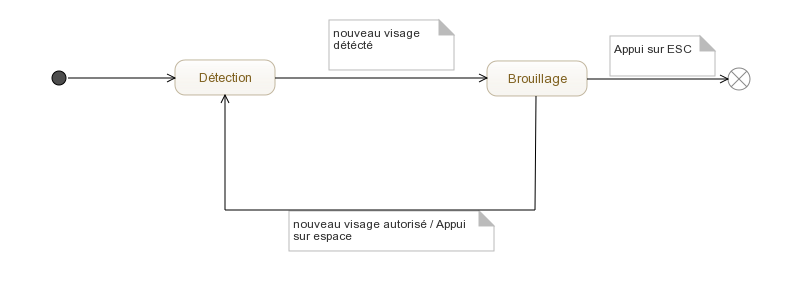
\includegraphics[width=\textwidth]{diag.png}
			\caption{Diagramme d'état du brouilleur}
		\end{center}
		\end{figure}
	\end{frame}
	
	
	\begin{frame}
	\frametitle{Conclusion}
	\begin{alertblock}{Améliorations possibles}
   	\rightskip=0pt\leftskip=0pt
	\begin{itemize}
		\item Détection des visages penchés 
		\item Reconnaître un visage précis
	\end{itemize}
	\end{alertblock}
	\begin{alertblock}{Pas de difficultés particulières}
   	\rightskip=0pt\leftskip=0pt
	\end{alertblock}	
	\end{frame}
\end{document}






